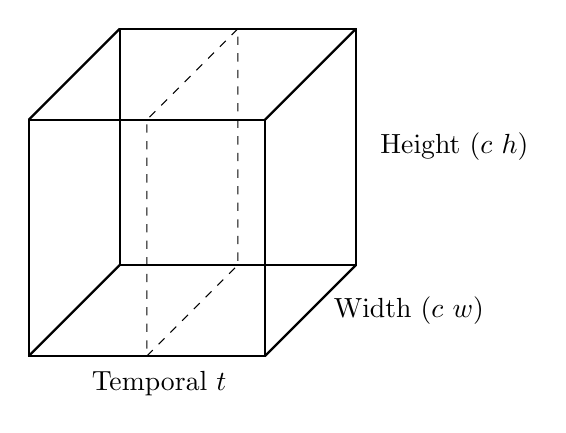
\begin{tikzpicture}
    % variables
    \def\cubeWidth{3}
    \def\cubeHeight{3}
    \def\cubeDepth{3}
    \def\slicePosition{1.5}

    % Cube points
    \coordinate (A) at (0, 0, 0);
    \coordinate (B) at (\cubeWidth, 0, 0);
    \coordinate (C) at (\cubeWidth, \cubeHeight, 0);
    \coordinate (D) at (0, \cubeHeight, 0);
    \coordinate (E) at (0, 0, \cubeDepth);
    \coordinate (F) at (\cubeWidth, 0, \cubeDepth);
    \coordinate (G) at (\cubeWidth, \cubeHeight, \cubeDepth);
    \coordinate (H) at (0, \cubeHeight, \cubeDepth);

    % Draw cube
    \draw[thick] (A) -- (B) -- (C) -- (D) -- cycle;
    \draw[thick] (E) -- (F) -- (G) -- (H) -- cycle;
    \draw[thick] (A) -- (E);
    \draw[thick] (B) -- (F);
    \draw[thick] (C) -- (G);
    \draw[thick] (D) -- (H);

    % Draw slice in middle
    \draw[dashed] (\slicePosition, 0, \cubeDepth) -- (\slicePosition, 0, 0) -- (\slicePosition, \cubeHeight, 0) -- (\slicePosition, \cubeHeight, \cubeDepth) -- cycle;

    % Axes
    \node at (0.5, -1.5, 0) {Temporal $t$}; 
    \node at (\cubeWidth + 1.25, \cubeHeight/2, 0) {Height $(c\ h)$};
    \node at (\cubeWidth + 1.25, 0, \cubeDepth/2) {Width $(c\ w)$};
\end{tikzpicture}